\documentclass[a4paper,twocolumn]{revtex4-1} %
\usepackage{amsmath}
\usepackage{graphicx}
\usepackage{braket}
\usepackage{comment}
\usepackage{hyperref}
\usepackage{soul,color}
\usepackage{cleveref}
%\usepackage{stfloats} % table on both columns
\usepackage[toc,page]{appendix}


\newcommand{\da}{\downarrow}
\newcommand{\ua}{\uparrow}
\newcommand{\ad}{\hat{a}^\dagger}
\newcommand{\an}{\hat{a}^{}}
\newcommand{\bd}{\hat{b}^\dagger}
\newcommand{\bn}{\hat{b}^{}}
\newcommand{\sd}{\hat{\sigma}^{+}}
\newcommand{\sn}{\hat{\sigma}^{-}}
\newcommand{\mbf}[1]{\mathbf{#1}}
\newcommand{\del}{\hat{\Delta}^{}}

\newcommand{\dm}{\widetilde{{\Delta}^{}}}
\newcommand{\A}{\mathbf{A}}
\newcommand{\B}{\mathbf{B}}

\newcommand{\EPF}{\ket{\text{EP-F}}}
\newcommand{\EP}{\ket{\text{EP}}}
\newcommand{\PP}{\ket{\text{PP}}}
\newcommand{\tPS}{\ket{\text{2P}}}
\newcommand{\tPF}{\ket{\text{2P-F}}}

\newcommand{\az}[1]{{\color{magenta}{#1}}}
\newcommand{\jk}[1]{{\color{red}{#1}}}
\newcommand{\pk}[1]{{\color{blue}{#1}}}
\newcommand{\q}[1]{{\color{cyan}{#1}}}

\newcommand{\symset}{\mathcal{S}}
\newcommand{\cntset}{\mathcal{P}} 
\newcommand{\indset}{\mathcal{I}} 

\newcommand{\maptoN}{{{\mathcal{M}}}_{N-1 \mapsto N}}
\newcommand{\maptoNa}{{\mathcal{M}}_{N-2 \mapsto N-1}}

\newcommand{\kb}{\ket{0}\!\bra{0}}
\newcommand{\klb}{\ket{\lambda}\!\bra{0}}
\newcommand{\kbl}{\ket{0}\!\bra{\lambda}}
\newcommand{\klbl}{\ket{\lambda}\!\bra{\lambda}}

\graphicspath{{./figs/}}
\usepackage{float}

\begin{document}

\title{Charge transport in organic microcavities: phonon-assisted zener tunnelling under strong light-matter coupling}

\author{M. Ahsan Zeb}
\affiliation{SUPA, School of Physics and Astronomy, University of St Andrews, St Andrews, KY16 9SS, United Kingdom}
\author{Peter G. Kirton}
\affiliation{SUPA, School of Physics and Astronomy, University of St Andrews, St Andrews, KY16 9SS, United Kingdom}
\author{Jonathan Keeling}
\affiliation{SUPA, School of Physics and Astronomy, University of St Andrews, St Andrews, KY16 9SS, United Kingdom}
\date{\today}

\begin{abstract}
Due to the coupling between electronic and vibrational states of organic molecules,
strong matter-light coupling in organic microcavities results
in a distribution of vibrationally excited states
 for the ground electronic state of a molecule.
These vibrations can assist zener tunnelling (charge transfer) 
under a moderate applied electric field.
The electron-hole pairs created this way
add up excitations to the coupled cavity-electronic subsystem when they combine to make excitons,
which in turn keeps the probability of excited vibrational states
high.
%This positive feedback makes the sustainable ...?
%The reverse is also true so we have a dynamical equilibrium between the two.
% and an equilibrium carrier concentration
%The vibrational distribution in the ground electronic state that triggers all this depends on the number of excitations in the cavity-electronic subsystem: the more the excitations, the higher the probability of having more vibrations....?????
\end{abstract}

\maketitle

\section{Intro}
The charge current in an organic semiconductor device
depends not only on the charge transport properties of
 the organic material involved but also on
  the injection and extraction properties of the contacts
  for it.
  The terms used for the two extremes ---  `space charge limited current'
 and `injection/contact limited current' ---
 are self-explanatory.
 When the current is injection limited,
 the current is lower than what the organic material allows.
In such a case,
%imagine we have a source of charge carriers in the bulk of organic material;
%for instance, 
creating pairs of mobile electrons and holes
by
shining light of appropriate wavelength (photoexcitation+charge transfer) or 
applying a sufficiently strong electric field (Zener tunnelling) can increase the current 
(assuming the extraction of charges is efficient and does not limit it).

Even for a %moderate 
HOMO-LUMO gap $E_g$ of $\sim2$eV,
Zener tunnelling needs a gigantic electric field strength
( $\sim 2\times10^{7}?$ V/cm)
 to promote an electron from HOMO of a molecule to
 LUMO of another one closed by (at a distance $\sim1$nm).
 The intramolecular vibrations in organic molecules
 involve stiff bonds so the energies of their vibrational quanta 
 are relatively large $\sim 0.1-0.35$eV. 
 They can assist the Zener tunnelling provided they are sufficiently excited.
 But, at ambient temperature ($k_bT=0.025$eV), 
 the molecules virtually stay in the ground vibrational state.
 Fortunately, these %intramolecular
  vibrational modes are coupled
  to the molecular electronic states, evident from
  the vibrational peaks in the optical absorption
   and emission spectra, 
   as explained by the Franck-Condon principle.
  That is, with a certain probability given by the Franck-Condon factor, photon absorption and emission can take to the excited vibrational states from the ground vibrational state in the excited and ground electronic manifolds respectively. 
 
 In an organic microcavity in the the strong coupling regime, the light-matter coupling leads to 
 a coherent energy exchange between the cavity and molecules
  making hybrid light-matter particles, polaritons.
 \hl {We show for the first time that},
   in such a case, 
  the simultaneous presence of the electron-photon and electron-phonon couplings, $\omega_R$ and $\lambda_0$, means that
   the excited vibrational states
   in the ground electronic manifold acquire a sizeable probability
  depending on
   these couplings
     and the vibrational frequency $\omega_v$,
     and can assist the Zener tunnelling,
      making it possible at far weaker applied electric fields.
    We present model calculations of incoherent charge transport in organic microcavities in the strong coupling regime and
explain recent experiments showing remarkably enhanced charge transport in metal-metal organic microcavities.
  
 
    
 
 
 
 




  
 
 
 
 
  


\section{Model}

  \begin{comment}
 The charge transport in (most disordered?) organics is via incoherent hopping between molecules. 
 Considering only two relevant electronic levels of organic molecules, HOMO and LUMO, with a single spin,
 the molecules %under usual circumstances 
 are
 either neutral with a single electron in HOMO or LUMO, 
 or have a charge, an extra electron in LUMO or a hole in HOMO.
  The electrons hop between HOMOs or LUMOs of
   neighbouring molecules to constitute hole or electron current.
% Shining light or applying a very strong electric field can create mobile electron hole pairs that would increase the current in an injection limited device as described above.
Under usual circumstances,
\end{comment}

Organic molecules are %modelled as having 
assumed to have two electronic levels with a single harmonic vibrational mode that is coupled to these electronic states (usual electron-phonon coupling). 
The cavity is %modelled as having 
assumed to have a single photon mode.


A molecule has four possible (spinless) electronic configurations:
\\{\it (i)} $\phi$ (both HOMO and LUMO empty), 
\\{\it (ii)} D (both HOMO and LUMO filled)
\\{\it (iii)} $\da$ (HOMO filled, LUMO empty), and 
\\{\it (iv)} $\ua$ (HOMO empty, LUMO filled).

D and $\phi$ do not couple to the cavity while $\da$ and $\ua$ do. 
We treat cavity along with all molecules in $\da$ or $\ua$ 
quantum mechanically using the rotating wave approximation for the coupling between them.
The rest of the molecules in D or $\phi$, and the electron hops 
between molecules or between contacts and molecules
are treated at classical level.
An electron hopping induces transitions between the quantum states as do the other dissipative processes like photon leakage and exciton decay.
We compute amplitudes for all possible quantum transitions 
and calculate respective transition probabilities
by weighing with a penalty function for their 
relevant classical hops.
Using usual rejection-free Monte Carlo rules, we select a transition at random and change the quantum and classical states accordingly.

\subsection{What is special?}
What is really interesting is that, in the strong coupling regime, the  electron hopping from HOMO of a molecule to the LUMO of its neighbour can be assisted by the vibrations that exist due to simultaneous presence of %strong light-matter coupling and 
vibronic coupling.

We do not explicitly include the vibrational states in quantum mechanically described subsystem. 
However, the probability distribution of vibrational states for molecules in $\da$ state is calculated quantum mechanically 
(see Fig.~\ref{fig:nv}, for example) and used to calculate the rates for classical hops.
This probability distribution can be very different than the thermal one, and if it is sufficiently large for excited vibrational states it
plays a vital/paramount role in the charge transport under applied bias.
For example, 
\\{\it(i)} for two neighbouring molecules in $\da$, 
the vibrations can assist the zener tunnelling by reducing the 
minimum applied field required for the process.
\\{\it(ii)}
these vibrations can enhance the inter-molecule HOMO-HOMO or LUMO-LUMO 
hop rates just like a higher temperature would~\cite{kudinov96}.


\begin{figure}[htpb]
  \centering
  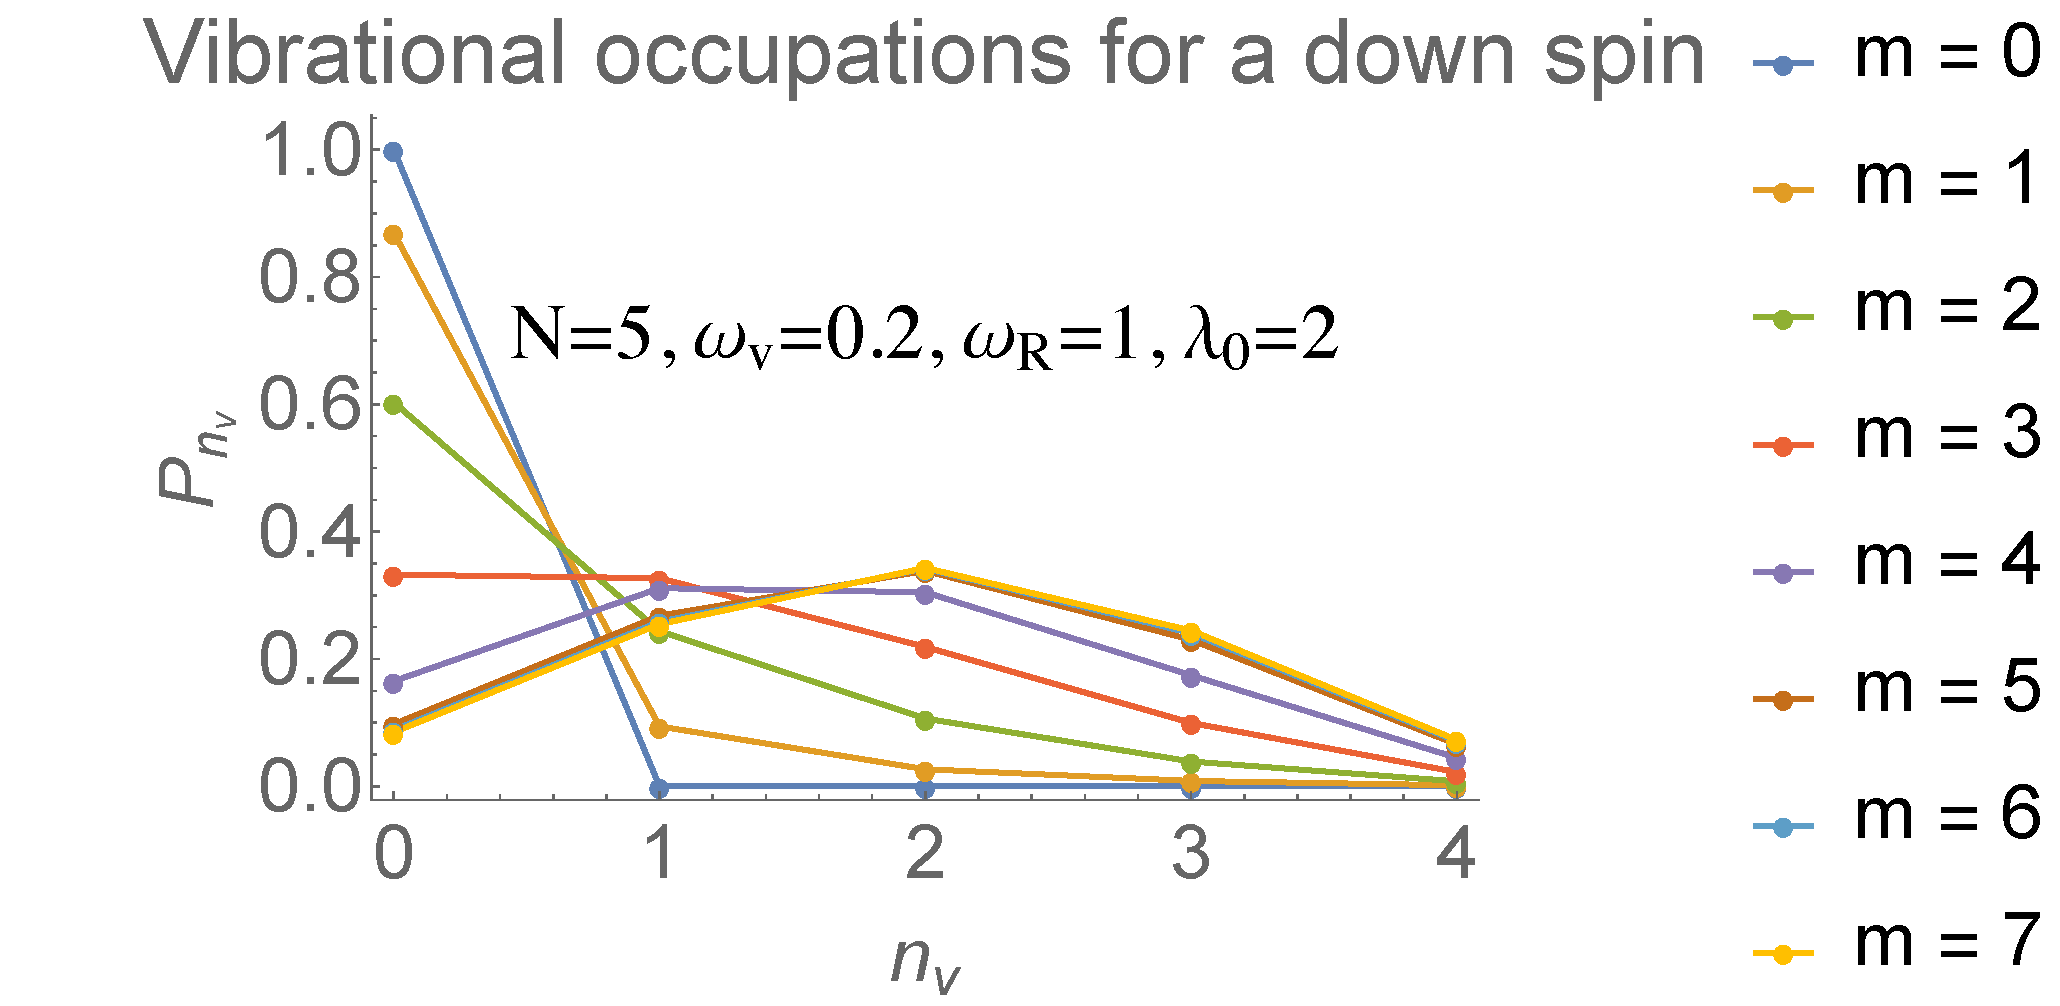
\includegraphics[width=1\columnwidth]{plot-n5}
  \caption{Probability distribution of vibrational states of a molecule in ground electronic state for different number of excitations $m$ in the system. 
 \label{fig:nv}}  
\end{figure}


\section{Hopping processes}

\subsection{Bulk processes}

An electron can jump from a molecule to its neighbour.
There are several possible ways this can occur: HOMO-HOMO, LUMO-LUMO, LUMO-HOMO and HUMO-LUMO.

\begin{itemize}
\item{D hops:}
when the initial site is doubly occupied and the final site is singly occupied,
this will be called a D hop, as the final site would become a D.
\item{$\phi$ hops:}
when the initial site is unoccupied and the final site is singly occupied,
this will be called a $\phi$ hop, as the final site would become a $\phi$.

\item{(D,$\phi$) creation:}
when the jump occurs between two singly occupied sites,
a pair of  D and $\phi$ is created.

\item{(D,$\phi$) annihilation:}
when the jump occurs between a D and $\phi$ pair, 
two singly occupied sites are created and the pair is annihilated.

\end{itemize}


\subsection{Contact processes}

An electron can jump from a molecule to a contact or vice versa.

\begin{itemize}
\item{D/$\phi$ creation:}
when the initial site is singly occupied, an electron can jump from the contact to it and make it D or it can jump from the molecule to the contact and make it a $\phi$.

\item{D/$\phi$ annihilation:}
It's just the reverse of the D/$\phi$ creation processes, where an initial D or $\phi$ becomes singly occupied when an electron jumps to or from it. 
\end{itemize}

%\subsection{Exciton decay and cavity losses} A photon leakage from the cavity or an exciton decay take remove an excitation so $m$ changes by -$1$. This does not involve any classical hops but a change in the quantum state.


\section{Classical hops induce quantum transitions}

Let's call $N$ and $m$ to the number of (singly occupied) sites
and number of (conserved) excitations in the quantum sub-system.
Whenever any of the processes outlines above happens at any site(s), via any allowed channels (HOMO-HOMO, LUMO-LUMO, etc.),
it can accompany a 
change in %the number of singly occupied sites $N$, and number of excitations $m$.
$(N,m)$.
There is a change in the quantum state of the coupled light-matter system and the new state lives in the subspace of the Hilbert space corresponding to the new $(N,m)$.
\Cref{tab:bulk,tab:cont} show the possible channels and corresponding change in $(N,m)$ for all hop types described above.

\begin{table}[h]
\begin{center}
\begin{tabular}{ |c|c|c|c|c| } 
 \hline
 Bulk Process & \multicolumn{4}{|c|}{Change in (N,m)} \\
 \hline
$\kappa/\gamma$ %cavity/exciton losses
& \multicolumn{4}{|c|}{0,-1}\\
\hline
 &H-H & L-L & H-L & L-H\\ 
D/$\phi$ hops & 0,0 &0,0 & 0,1 & 0,-1\\ 
(D,$\phi$) creation & -2,-1 &-2,-1 & -2,0 & -2,-1\\ 
(D,$\phi$) annihilation & 2,1 &2,1 & 2,2 & 2,0\\ 
 \hline
\end{tabular}
\end{center}
\caption{Change in the number of active sites $N$ and excitations $m$ in the quantum system for bulk processes.\label{tab:bulk}}
\end{table}

\begin{table}[h]
\begin{center}
\begin{tabular}{ |c|c|c| } 
 \hline
Contact Process & \multicolumn{2}{|c|}{Change in (N,m)} \\
 &HOMO & LUMO\\ 
\hline
D creation & -1,-1 & -1,0\\ 
D annihilation & 1,1 & 1,0\\ 
$\phi$ creation & -1,0 & -1,-1\\ 
$\phi$ annihilation & 1,0 & 1,1\\ 
 \hline
\end{tabular}
\end{center}
\caption{Change in the number of active sites $N$ and excitations $m$ in the quantum system for contact processes.\label{tab:cont}}
\end{table}



%\subsection{Dynamics}

\subsection{The state of the system}
The overall `state' of the system
at any time is described by
the set of D and $\phi$ sites,
$(N,m)$, and the quantum state $\ket{\psi}_{N,m}$.
$\ket{\psi}_{N,m}$ can be a superposition of eigenstates in a given degenerate sector of the spectrum of the instantaneous quantum subsystem.

\subsection{How the state evolves in time}
We find all possible ways a hopping process can occur. 
For example, every D that has a singly occupied neighbour, can hop to it, every D that has a $\phi$ as neighbour can combine with it and both get annihilated, every pair of neighbours that are singly occupied can create a (D,$\phi$) pair, etc.

Let's label all such possible ways of all hops for all channels 
by $\{\alpha\}$.
We calculate their transition matrices $H_t^{\alpha}$,
and %the unitary transformation matrix $U_{N_{\alpha},m_{\alpha}}$ (set of eigenvectors, columns-wise) that diagonalise $H_{N_{\alpha},m_{\alpha}}$ 
the set of eigenstates $\{ \ket{\phi_i} \}$ of 
the Hamiltonian
  for $(N_{\alpha},m_{\alpha})$, the final number of sites and 
  excitations for hop $\alpha$.
  The amplitudes for the transition from 
  the current quantum state to the
  final quantum states for hop $\alpha$
  is 
\begin{gather}
  C_{\alpha,i} = \bra{\psi_{N,m}}H_t^{\alpha}\ket{\phi_{N_{\alpha},m_{\alpha}}^i}.
\end{gather}

After hop $\alpha$ we will quickly lose coherence between eigenstates 
of $H_{N_{\alpha},m_{\alpha}}$ with different 
energies, but
there are multiple degenerate sectors in the spectrum 
and 
 the coherence persists between
 eigenstates lying in the same degenerate sector.
So, in Monte Carlo, we consider quantum jumps to all possible degenerate sectors
instead of individual states.
Suppose $\{\beta\}$ labels the degenerate sectors
of $H_{N_{\alpha},m_{\alpha}}$, then
the probability that we jump to sector $\beta$
is
\begin{gather}
P_\beta = f(\Delta E_{\alpha,\beta}) \times \sum_{i\in\beta} |C_{\alpha,i}|^2,
\end{gather}
where 
$\Delta E_{\alpha,\beta}$ the net change in energy
for the quantum transition to degenerate sector $\beta$ with classical hop $\alpha$
 including the change due to the applied electric field,
 and 
 $f(\Delta E_{\alpha,\beta})$ is a penalty function given by,
\begin{equation}
\nonumber
  f(x)=\begin{cases}
    1, & \text{if $x<0$}.\\
    e^{-x/{T}}, & \text{otherwise}.
  \end{cases}
\end{equation}
Here, the environment is assumed to be in thermal equilibrium at
a temperature $T$.

Suppose, we stochastically select 
classical hop $\alpha$ with quantum transition to degenerate sector $\beta$,
 then
the final state is
\begin{gather}
\ket{\psi_{N_{\alpha},m_{\alpha}}}= \sum_{i\in\beta} C_{\alpha,i} \ket{\phi_{N_{\alpha},m_{\alpha}}^i}.
\end{gather}
Once we update the overall state, i.e., the set of $D$ and $\phi$, $(N,m)$ and the quantum state, the cycle starts again.
%We calculate transition matrices for all such possible ways of all hops for all channels, then compute the probabilities of all possible quantum transitions and weigh them with a penalty function for the classical hops that depends on the energetic difference between the initial and final electron state, applied electric field and intermolecular distance, etc.

The details of how the transition matrices are calculated and the Monte Carlo dynamics is performed
is given in the appendix. 



\section{Explaining experiments}

\subsection{Experimental findings}
Experiments are performed on metal-metal microcavities, with Al mirrors and MEH-PPV as active organic material (in PMMA matrix?). 
The fermi level of Al is at $\sim -4.2$eV and 
HOMO/LUMO of MEH-PPV are at $\sim -2.7,-5.1$eV.
Experimentalists think that there exists a moderate energy barrier for electron injection and a large barrier for hole injection such that the charge transport occurs only via electrons in this system because the holes injection at the anode is blocked.

{\it Observations:}
In the experiments, it is found that, at average electric fields $\sim 10^6$V/cm, the current is 2-3 orders of magnitude higher in resonant cavities compared to the non-resonant ones. Further, there is electroluminescence in the resonant case even if the hole injection from the anode is absent due to a hole blocking layer there. No light emission is seen in the non-resonant cavities.

\subsection{Possible explanations}
\label{subsec:zener}
The observation of electroluminescence in resonant cavities means there is a constant supply of holes so they either enter from the cathode which is less likely, or they are produced in processes that create electron-hole pairs.
The average electric field in the experiments ($\sim 10^6 V/cm$) 
is too small in comparison to the 
$\Delta_{HOMO-LUMO}\sim 2eV$
 and this cannot induce the HOMO-LUMO hops alone.
 So, either one or both of the following can be at work.
 
 \begin{itemize}
 
 \item {\it(i)} 
 There are locations in the system/device 
 where the field is much stronger than the average value so that it is able to create (D,$\phi$) 
 pairs.
In the weak coupling regime/off-resonant cavities,
these (D,$\phi$) pairs are wasted via creation of excitons
close to their birth place and hence do not contribute significantly to the charge transport.
However, in the strong coupling regime/resonant cavities,
excitons created by them add up excitations in the coupled 
matter-light quantum subsystem, which allows the creation
of (D,$\phi$) pairs anywhere.
%Depending on the efficiency of this re-creation or effectively delocalisation of charge carriers (D and $\phi$),
This would effectively evenly distribute the charge carriers (D and $\phi$) which is much more likely to contribute to the current (and hence enhance the transport via increased carrier concentration as well as via avoiding electron traps, see somewhere below for how to avoid traps).
 
\item {\it(ii)} 
Due to the coupling between electronic and intramolecular 
 vibrational states, there is a sizeable probability of having enough 
 phonons/vibrational quanta 
 on an unexcited molecule ($\da$)
 that %the energetic difference between initial and final electron state for a HOMO-LUMO channel is easily overcome.
 the energy required for the hop from it to the LUMO of a neighbour molecule is available. That is, vibrational/phonon assisted zener tunnelling/charge transfer process becoming possible even at average strengths of bias fields that alone are not sufficient for this process (say, $\sim10^6$ V/cm). 

\end{itemize}

{\bf A Test: }
Whether this is the reason of higher currents in resonant cavities 
can be tested by blocking electron and hole injection from the 
contacts in a microcavity with no intrinsic holes to establish the 
strong coupling regime and exciting it with a laser above the exciton energy. 
Once the system is in strong coupling regime 
(with enough excitations to have a sizeable probability 
of phonons in the ground electronic state of molecules),
it can start creating (D,$\phi$) pairs and add excitations in the 
quantum system, which should then be sustained even if the laser 
drive is removed.


\subsection{Why resonant cavities allow more current? Is it enhanced injection or carrier generation?}

Note: If the cavity lowers the molecular levels, would not it be likely to lower the metallic levels too?!

Anyway, some tests:
\begin{itemize}
 
 \item {\it Test 1. }
If J-V characteristics of resonant cavities are similar
 to non-resonant ones at small applied bias (say, $\lesssim10^{3}V/cm$),
that means the injection barriers are not drastically different
in the two cases.
 
 \item {\it Test 2. }
A microcavity with electron and hole blocking layers at cathode and anode would stop any injection.
If the J-V characteristics of resonant cavities stay similar,
that would mean injection is not playing any role.

 \item {\it Test 3. }
Take a microcavity with excellent electron and hole injection, e.g., Ca cathode and Au anode with MeH-PPV.
At low fields where zener tunnelling is not possible even with vibrational assistance,
if the resonant cavities have higher currents,
that would mean carrier's mobility is enhanced (due to the vibrations resulting from strong coupling).

\end{itemize}


\subsection{What about the traps?}
It is well known that the mobility of holes is $\sim 3$ orders of magnitude higher than electrons in MEH-PPV (and other organic polymers??) due to deep trap states below the LUMO level~\cite{Zhang10}.
This difference in mobility pertains to hole-only and electron-only transport.
In the strong coupling regime, when the singly occupied sites can switch between HOMO and LUMO, an electron can avoid traps by going through HOMO and hence this alone is sufficient to increase the current due to increased mobility. 
But, it is not sustainable on its own as the excitations in the system are constantly dissipated via photon leakage and exciton decay, and an electron is unlikely to be extracted from HOMO at the cathode. 
{\bf This again means there is some source of excitations in the resonant cavities, as discussed in section~\ref{subsec:zener}. 
So, the combined effect of increased mobility due to avoiding traps and increased carrier concentration is likely to be the reason of orders of magnitude higher current in resonant cavities.}

\subsection{Photo assisted charge transfer}
Does not add excitations! Can't be the reason.










\bibliography{organic}




%This is a huge computational task so limit the size of the system we can treat.
%\appendix
\renewcommand{\theequation}{S\arabic{equation}}
\setcounter{equation}{0}
\renewcommand{\thefigure}{S\arabic{figure}}
\setcounter{figure}{0}
\setcounter{section}{0}

\clearpage

\onecolumngrid
\begin{center}
\textbf{\large Appendix: implementation details}

\vspace{0.4cm}

%{M.\ Ahsan Zeb, Peter G.\ Kirton and Jonathan Keeling} \\ \textit{SUPA, School of Physics and Astronomy, University of St Andrews, St Andrews, KY16 9SS, United Kingdom}\\ (Dated: \today)

\end{center}
\vspace{\columnsep}
%\twocolumngrid


%\title{Supplimentary Materials: Charge transport in organic microcavities: phonon-assisted zener tunnelling under strong light-matter coupling}

%\maketitle
\section{Overview}

\subsection{Nomenclature}
\begin{itemize}
\item D: doubly occupied site
\item $\phi$: empty/unoccupied site
\item Active: singly occupied site, $\da$ or $\ua$, that couples to the cavity.
\item Channels: H-H, L-L, L-H, H-L channels for electron jumps.
\item Bulk hopping parameters: $t_h$, $t_l$, $t_{lh}$, $t_{hl}$ for H-H, L-L, L-H, H-L channels.
\item Contact hopping parameters: $J_{h,R}$, $J_{l,R}$, $J_{h,L}$, $J_{l,L}$ for RC-H, RC-L, LC-H, LC-L channels, where RC and LC stand for right and left contats.
\item Sites: molecules
\item classical hop: electron hop between molecules or contact and molecule, treated classically, i.e., no interference effects between different hops.
\item quantum transition: transition between eigenstates of the quantum mechanically described system, i.e., active sites coupled to the cavity.
\item Degenerate sectors: degenerate sectors in the energy eigenvalues of coupled light-matter system. 
\item Transition matrix: transition matrix due to a classical hopping process 
that gives the bare amplitudes for the quantum transitions for given initial and final states.
\item Penalty function: a penalty function suppressing the transition rate by a Boltzmann factor if there is a positive energy cost for the transition. This is widely used in Monte Carlo simulations to allow, in a statistical way, the energy exchange between the system and the environment. 
\end{itemize}


\subsection{Steps in a MC iteration}
The Monte Carlo dynamics consist of iterations over the following steps.

%At every iteration, steps:\\
\begin{enumerate}
\item 
{\bf The sets of allowed sites for all kind of processes:}
From the overall state of the system
that gives
the sets of D, $\phi$ and active sites, 
the sets of sites or pairs of sites for various hopping processes
is calculated. Electron hops to the right and left are treated separately.
For example, suppose two neighbouring sites are found in D and $\phi$ sets
with $\phi$ on the right of the D in the lattice, 
then they are added to the list for (D,$\phi$) pair annihilation with electron hopping to the right.


\item
{\bf The transition matrices are calculated for all available sites and channels for allowed processes.}
For the quantum mechanically described active sites that are coupled to the cavity,
their order in the basis set does not have to be the same as in the lattice (position space)
and is taken into account when computing transition matrices for various processes.

\item
{\bf  The transition amplitudes are computed that are used with corresponding energetic penalties 
to find the transition rates.}
The energetic penalties consider all relevant changes in the energy, possible contributions are:
the difference between energies of initial and final quantum
and classical states (D has an energy $\omega_0$),
energetic barriers at the contacts, energy gain/lost due to the applied electric field,
and finally the vibrational energy of an active site for hops from it if vibrational assistance is included.

\item 
{\bf  A transition is selected stochastically and the quantum state and the sets of D, $\phi$ and $\mathcal{A}$ is changed accordingly.}
The time is advanced by a random selection of incremental time
from the exponential distribution decaying with the combined rate of all processes. 
After the transition, it is assumed that the interaction with the environment, low energy vibrations,
quickly relaxes the system to its lower polariton state.
So the state is changed accordingly and the loop restarts again from point $1$ above.

\end{enumerate}



\section{Transition Matrices}
%\subsection{Definitions}
%$\mathcal{A}_{n}$ Index in the list of active sites.
%$\mathcal{L}_{n}$ Index in the list of lattice sites.
%Spin sectors:\\
For $N$ active sites and $m$ excitations,
the basis states are made of sets of basis with $k\in [0,min(m,N)]$ sites in $\ua$ state
and indexed in lexicographic order.
The transition matrix maps are calculated for each of such set and combined to make full matrix.


\subsection{D hops right/left}
An electron hops from a D site to an active site.
The active site becomes D and vice versa, the index of the initially active site is assigned to the new active site. 
\\Transition matrix elements:\\
The basis states that have final site $\ua$ would allow 
an electron hopping to its HOMO level and create a D.
This hop leaves the initially D site in $\ua$ (channel 1) or $\da$  (channel 3).
Similarly,
the basis states that have final site $\da$ would allow 
an electron hopping to its LUMO level and create a D.
This hop leaves the initially D site in $\da$ (channel 2) or $\ua$  (channel 4).



\subsection{$\phi$ hops right/left}
An electron hops from an active site to a $\phi$.
The active site becomes $\phi$ and vice versa, the index of the initially active site is assigned to the new active site. 
\\Transition matrix elements:\\
The basis states that have the active site $\ua$ would allow 
the electron hopping from it and change it to $\phi$.
This hop makes the initially $\phi$ site in $\ua$ (channel 2) or $\da$  (channel 3).
Similarly,
The basis states that have the active site $\da$ would allow 
the electron hopping from it and change it to $\phi$.
This hop makes the initially $\phi$ site $\da$ (channel 1) or $\ua$  (channel 4).

\subsection{(D,$\phi$) creation: }
For two adjacent active sites,
we can have four configurations:
$(\ua,\da)$, $(\da,\ua)$,$(\ua,\ua)$,$(\da,\da)$ with left and right sites in (left,right) order.
These will make (D,$\phi$) pair with D on the left 
with the hopping of an electron from right to left 
via H-H, L-L, L-H, and H-L channels.
Similarly,
a (D,$\phi$) pair with D on the right is created from these configurations
with the hopping of an electron from left to right
via L-L, H-H, L-H, and H-L channels, respectively.
\\Transition matrix elements:\\
The map between basis states of initial and final Hilbert spaces
$\mathcal{H}_{N,m}$ and $\mathcal{H}_{N-2,m^\prime}$, 
where $m^\prime=m,m,m-1,m-2$ for H-H, L-L, L-H, H-L channels,
can be calculated by starting from the final basis states in $\mathcal{H}_{N-2,m^\prime}$ 
and inserting the two active sites
at their position in desired configuration ($(\ua,\da)$, etc.) to make the initial basis state.
Let's call the combination of $k$ ($k\in [0,min(m,N)]$) $\ua$ sites in the latter $set$ and its lexicographic index
$x$ in this $k-\ua$-sector, then
\begin{eqnarray*}
x = c^N_ k - 
   \sum_{p=0}^{k-1}c^{N - set(p)}_{ k - p},
   %   c^n_r &=& \frac{n!}{r!(n-r)!}.
\end{eqnarray*}  
 where, $c^n_r = {n!}/{r!(n-r)!}$.
  This index is then shifted up by an amount 
$\sum_{k^\prime=0}^{k-1} c^N_{k^\prime}$ to obtain the absolute index of the considered basis state.









\subsection{(D,$\phi$) annihilation: }
This is just the reverse of (D,$\phi$) creation described above where two active sites are created
from a pair of D and $\phi$. The freshly added active sites are given the indices $N+1,N+2$
and the map for the transition matrix is computed just like (D,$\phi$) creation case.
Since the electron hopping does not occur on active sites in this case,
a single (D,$\phi$) pair can be used to calculate the transition matrix and amplitudes.


\subsection{ D/$\phi$ creation at contacts: }
If the site adjacent to a contact is active, 
it can gain or loose an electron via hopping from/to the contact to become a D or $\phi$.
The basis states with this site $\da$ 
can get an electron from the contact (hopping parameter $J_{l,R/L}$; $R and L$ for right and left contacts)
and become D or it can loose the electron to the contact (hopping parameter $J_{h,R/L}$)
and become $\phi$
resulting in one less active site $N\rightarrow N-1$ and $m$ unchanged.
That is, the final state is in $\mathcal{H}_{N-1,m}$. 
The transition matrix map is obtained simply by starting with the basis in $\mathcal{H}_{N-1,m}$,
inserting an $\da$ in correct position to make the state in $\mathcal{H}_{N,m}$,
and calculating its lexicographic index.
Similarly, the basis states with this active site $\ua$ 
are linked via $J_{h,R/L}$ and $J_{l,R/L}$ to 
the basis in $\mathcal{H}_{N-1,m}$
for creation of D and $\phi$ respectively.
The transition matrix map is calculated the same way.


\subsection{ D/$\phi$ annihilation at contacts: }
These are just the reverse of D/$\phi$ creation at the contacts.
A D or $\phi$ site adjacent to a contact becomes active on loosing or gaining an electron to/from it.
Starting with D, 
the basis states in $\mathcal{H}_{N,m}$
are linked via $J_{l,R/L}$ ($J_{h,R/L}$) to 
the basis in $\mathcal{H}_{N+1,m^\prime}$ with $m^\prime=m\,(m+1)$
with this site being $\da$ ($\ua$).
For a $\phi$, 
the same transition map results with $J_{l,R/L} \leftrightarrow J_{h,R/L} $.

\subsection{cavity losses, $\kappa$}
A photon leaking out of the cavity reduces the number of excitations $m \rightarrow m-1$.
If $m-1 \geq N$, the transition matrix equals identity with the new basis with one less photon but the same combinations of $\da,\ua$ sites.
Otherwise, sectors with $m$ $\ua$ sites is no longer available, but
the rest of the basis with up to $m-1$ $\ua$ 
have a one-to-one map with the final basis that now have one less photon.

\subsection{exciton losses, $\gamma$}
An excited molecule decaying non-radiatively also means $m \rightarrow m-1$.
But, now the map from initial basis to the final depends on which molecule decays.
Suppose, $n$-th molecule decays, then we start with the final basis for 
$\mathcal{H}_{N-1,m-1}$,
insert a $\da$ at the $n$-th position and compute 
the lexicographic index of the starting basis for this process.




\end{document}

\begin{acknowledgments}
  JK and MAZ acknowledges financial support from EPSRC program ``Hybrid
  Polaritonics'' (EP/M025330/1).  PGK acknowledges support from EPSRC
  (EP/M010910/1). 
\end{acknowledgments}

